\documentclass[12pt]{article}

\usepackage[left=2.5cm,right=2cm,top=2cm,bottom=2cm]{geometry}
\setlength{\parindent}{0mm}

\usepackage{float}

\usepackage{parskip}
\usepackage[document]{ragged2e}
\usepackage{babel}
\usepackage[utf8]{inputenc}
\usepackage{amsmath,amsthm,mathtools}
\usepackage{amsfonts,amssymb,latexsym}
\usepackage{enumerate}
\usepackage[dvips,usenames]{color}
\definecolor{RojoAnayelRey}{rgb}{1,.25,.25}
\usepackage{tikz}
\usepackage[bookmarks=true,
            bookmarksnumbered=false, % true means bookmarks in 
                                     % left window are numbered                         
            bookmarksopen=false,     % true means only level 1
                                     % are displayed.
            colorlinks=true,
            linkcolor=blue]{hyperref}
            
\usepackage[T1]{fontenc}

\title{Tareas varias voluntarias}

\author{David Cabezas Berrido}

\date{}

\begin{document}
\maketitle

\section{Resolución de sistemas de ecuaciones en R}

La función
\href{https://www.rdocumentation.org/packages/base/versions/3.6.2/topics/solve}{\texttt{solve}}
de R, sirve para resolver sistemas de ecuaciones lineales. En
concreto, ecuaciones del tipo $ax=b$, donde $a$ es una matriz cuadrada
real o compleja (la matriz de coeficientes del sistema) y $b$ una
matriz o un vector real o complejo. La función \texttt{solve(a,b)}
devuelve la matriz o vector $x$ que resuelve el sistema. Si se omite
el parámetro $b$, se toma la matriz identidad, por lo que la función
devuelve la inversa de $a$.

\begin{figure}[H]
  \centering
  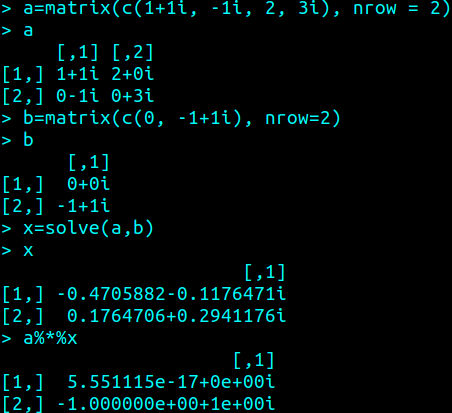
\includegraphics[width=80mm]{imgs/solve}
  \caption{Ejemplo de uso de solve para resolver un sistema lineal complejo de dos ecuacioness.}
\end{figure}

En este ejemplo definimos una matriz compleja $2\times 2$ $a$, un
vector complejo $b$ con 2 componentes, llamamos a la función solve
para resolver el sistema y asignamos el resultado a la variable
$x$. Después comprobamos que efectivamente $x$ satisface la ecuación
$ax=b$.

\section{El paquete gráfico ggplot2}

\texttt{ggplot2} es un paquete gráfico de R. Según
\href{https://ggplot2.tidyverse.org/index.html}{https://ggplot2.tidyverse.org/index.html},
está basado en el libro \emph{The Grammar of Graphics}, de Leland
Wilkinson. En la página \\
\href{https://www.rdocumentation.org/packages/ggplot2/versions/3.3.2}{https://www.rdocumentation.org/packages/ggplot2/versions/3.3.2}
se encuentra una guía de instalación, una Cheatsheet, una descripción
de las funciones del paquete y algunos tutoriales para dominarlo.

Probamos y explicamos un pequeño ejemplo encontrado en: \\
\href{https://www.datanovia.com/en/lessons/introduction-to-ggplot2/}{https://www.datanovia.com/en/lessons/introduction-to-ggplot2/},
en el que representamos en un diagrama de dispersión (esto lo hacemos
con
\href{https://www.rdocumentation.org/packages/ggplot2/versions/3.3.2/topics/aes}{\texttt{aes(x,y)}})
en el que representamos la longitud (eje $X$) y anchura (eje $Y$) de
los pétalos de las distintas flores. Elegimos un color y una forma
diferentes para cada clase. Seleccionamos manualmente los colores en
formato RGB hexadecimal: \#FF0000 sería el rojo más puro e intenso
posible, \#00FF00 el verde más puro y \#0000FF el azul puro.

\begin{figure}[H]
  \centering
  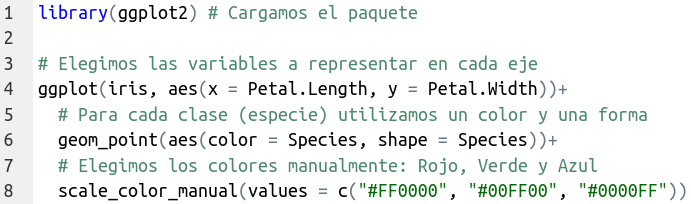
\includegraphics[width=120mm]{imgs/ggplot2-code}
  \caption{Ejemplo de gráfico con \texttt{ggplot2}.}
\end{figure}

Este es el gráfico que generamos:

\begin{figure}[H]
  \centering
  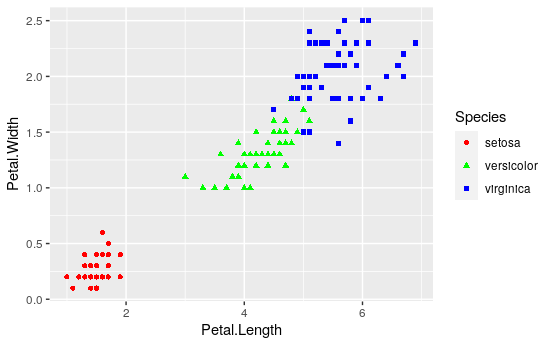
\includegraphics[width=120mm]{imgs/ggplot2-iris}
  \caption{Gráfico generado}
\end{figure}

\section{Método del codo para la selección del número de componentes
  principales}

El
\href{https://en.wikipedia.org/wiki/Elbow_method_(clustering)}{método
  del codo}, es una heurística que se utiliza para determinar el
número de clusters en un dataset. Consiste en representar la
proporción de varianza explicada en función del número de clusters y
escoger el número de clusters en el que se produzca el
\href{https://en.wikipedia.org/wiki/Knee_of_a_curve}{codo de la
  curva}.

Esta misma técnica se puede utilizar para elegir el número de
componentes principales para describir los datos, sólo hay que
representar la proporción de varianza acumulada por las $n$ primeras
componponentes principales como función de $n$ y elegir el valor de
$n$ con el código de la curva. También se puede hacer (como explica
\href{https://feliperego.github.io/blog/2016/05/31/Intro-To-Principal-Component-Analysis}{aquí})
sobre el porcentaje de varianza explicada por cada componente
princial, e identificar el valor de $n$ a partir del cual la varianza
explicada por cada posterior componente principal sea baja.

Ponemos como ejemplo el dataset de las concentraciones de elementos
químicos en muestras de vidrio del paquete ``archdata''. En lugar de
como gráfico de barras, cambiamos la prepresentación a líneas y puntos
para que sea más fácil identificar el codo de la curva.

\begin{figure}[H]
  \centering
  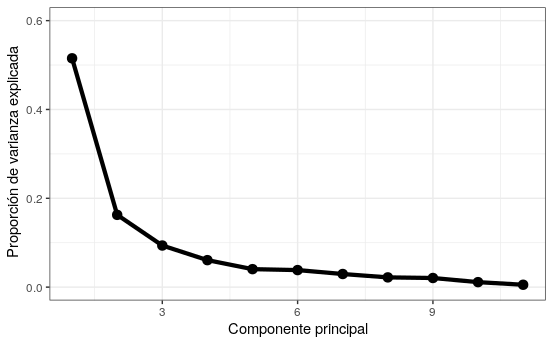
\includegraphics[width=120mm]{imgs/elbow}
  \caption{Curva de varianza explicada de cada componente principal.}
\end{figure}

\begin{figure}[H]
  \centering
  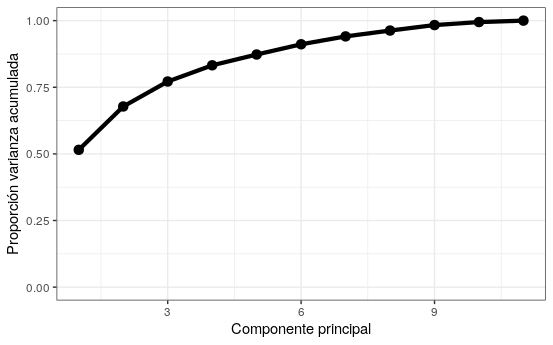
\includegraphics[width=120mm]{imgs/elbow-cumsum}
  \caption{Curva de varianza explicada acumulada de cada componente
    principal.}
\end{figure}

En ambas curvas, podemos identificar el codo para el valor 3 del
número de componentes principales.

\end{document}
